\documentclass[11pt,a4paper]{article}
\usepackage[margin=1in]{geometry}
\usepackage[T1]{fontenc}
\usepackage[utf8]{inputenc}
\usepackage{lmodern}
\usepackage{hyperref}
\usepackage{enumitem}
\usepackage{xurl}
\usepackage{tikz}
\usepackage{float}
\usetikzlibrary{arrows.meta, positioning, shapes.geometric}
\hypersetup{colorlinks=true,linkcolor=blue,urlcolor=blue}
\newcommand{\codepath}[1]{\path{#1}}
\tikzset{box/.style={rectangle,draw,rounded corners,align=center,inner sep=3pt,minimum width=36mm},line/.style={-Latex}}

\title{Phase-2 Deliverable: Golden Output Artifacts}
\author{SIT Engine Architecture}
\date{\today}

\begin{document}
\maketitle

\section{Technical Description}
Golden output artifacts are deterministic SIT outputs (\texttt{windows} and \texttt{summary}) tied to trace inputs, engine behavior, and schema version. They are the primary regression oracle for replay checks.

\section{Implementation Fulfillment}
Materialized by:
\begin{itemize}[leftmargin=*]
  \item replay harness: \codepath{Phase-2/tests/run_golden_suite.py},
  \item SIT engine: \codepath{Phase-2/sit_engine_phase1.py},
  \item export schema checks: \codepath{Phase-2/schema/v1.py},
  \item determinism verification: \codepath{Phase-2/tests/check_determinism.py}.
\end{itemize}
Runtime outputs are emitted as \codepath{*_windows.csv} and \codepath{*_summary.json}. Adapter execution metadata is emitted via \codepath{adapter\_meta.json} in \codepath{Phase-2/riscvbench.py}.

\section{Design \& Architecture}
Given fixed inputs (trace, residency mask, window size, expected work rate), replay outputs are expected to be byte-stable across reruns. Artifact lineage is preserved through manifest dataset version fields and embedded summary metadata.

Current governance gap: formal packaging policy for mandatory versus optional artifact formats (CSV/JSON/Parquet) is not yet codified.

\subsection*{Function Flowchart}
\begin{figure}[H]
\centering
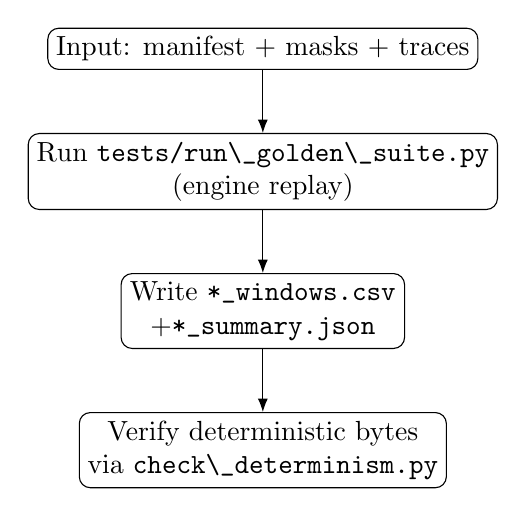
\begin{tikzpicture}[node distance=8mm and 12mm]
\node[box] (a) {Input: manifest + masks + traces};
\node[box, below=of a] (b) {Run \codepath{tests/run\_golden\_suite.py}\\(engine replay)};
\node[box, below=of b] (c) {Write \codepath{*_windows.csv}\\+\codepath{*_summary.json}};
\node[box, below=of c] (d) {Verify deterministic bytes\\via \codepath{check\_determinism.py}};
\draw[line] (a) -- (b);
\draw[line] (b) -- (c);
\draw[line] (c) -- (d);
\end{tikzpicture}
\caption{Golden Output Artifact Flow}
\end{figure}

\end{document}
